\chapter{Kunstmatige Netwerken}
Enkele notaties:
\begin{itemize}
    \item De neuronen van het netwerk worden aangeduid met de letters $x$, $y$ of $z$. Deze worden genummerd door een onderindex $i$.
    \item De verbindingen in de graaf krijgen geen apart symbool. Het gewicht van de tak die van $x_i$ naar $x_j$ gaat noteren we als $w_{ij}$; in het geval dat er geen verbinding is, is $w_{ij} = 0$.
    \item De uitvoer van neuron $x_i$ duiden we aan met $u_{i}$.
    \item Een rij getallen die een vector voorstellen worden geschreven met een vette letter: $\textbf{v} = (v_1, ... v_n)$. 
\end{itemize}
\begin{figure}[ht]
    \centering
    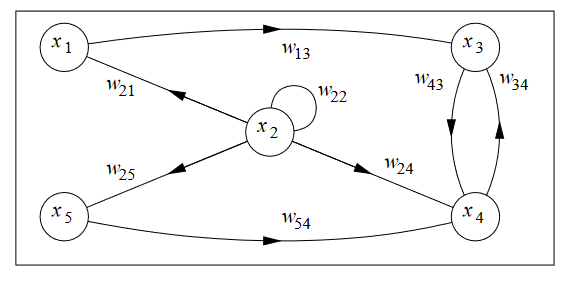
\includegraphics[width=\textwidth]{neuraal_net}
    \caption{Schema van een neuraal net.}
    \label{}
\end{figure}

Een neuraal net is vaak ingedeeld in verschillende lagen, waarin elke laag een verschillende functie heeft. De nulde laag bestaat uit de invoercellen. Er zijn twee vormen:
\begin{enumerate}
    \item \textbf{Gesloten gelaagde netten}: Er zijn enkel verbindingen mogelijk tussen opeenvolgende lagen van het net. Van laag $k$ naar $k + 1$, of met terugkoppeling, van $k + 1$ naar $k$.
    \begin{figure}[ht]
        \centering
        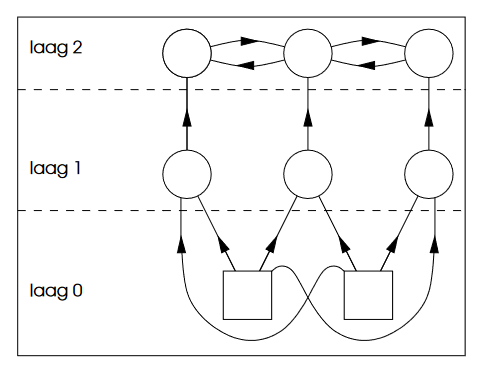
\includegraphics[width=0.5\textwidth]{gesloten_gelaagd_net}
        \caption{Gesloten gelaagd net}
        \label{}
    \end{figure}
    \item \textbf{Open gelaagde netten}: Er zijn verbindingen mogelijk tussen twee willekeurige lagen.
    \begin{figure}[ht]
        \centering
        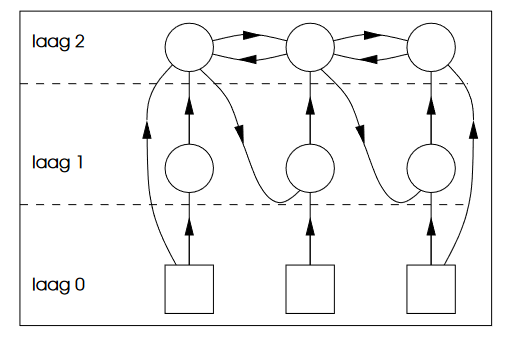
\includegraphics[width=0.5\textwidth]{open_gelaagd_net}
        \caption{Open gelaagd net}
        \label{}
    \end{figure}
\end{enumerate}

\section{Artificiële neuronen}
Er zijn drie belangrijke kenmerken die kunstmatige neuronen kunnen onderscheiden:
\begin{enumerate}
    \item De \textbf{reactiefunctie}: deze geeft aan wat de uitvoer is in functie van de invoer.
    \item De \textbf{uitvoeringsmethode}: beschrijft hoe de verandering in uitvoer wordt doorgevoerd. Twee opties:
    \begin{enumerate}
        \item Direct.
        \item Wachten op een extern signaal (bv. Hopfieldnetten).
    \end{enumerate}
    \item De \textbf{tijd}: vaak wordt er verondersteld dat alle wijzigingen ogenblikkelijk gebeuren.
\end{enumerate}

\section{TLU's}
TLU = Threshold Logic Unit

\begin{itemize}
    \item Wordt gebruikt in binaire netwerken.
    \item De werking van een neuron wordt bepaald door een drempelwaarde, die voor elke neuron verschillend kan zijn.
    \item Als de drempelwaarde van neuron $x_i$ gelijk is aan $T_i$, wordt de uitvoer gegeven door
    $$u_i = \begin{cases}
        1 \quad \hbox{als}\quad \sum_jw_{ji}u_j \geq T_i \\
        0 \quad \hbox{als}\quad \sum_jw_{ji}u_j < T_i
    \end{cases}$$
    \alert Ook mogelijk om extra neuron $x_0$ in te voeren, die verbonden is met elke andere neuron met gewicht $w_{0i} = -T_i$. Op die manier wordt de reactiefunctie gelijk voor alle neuronen:
    $$f(r) = \begin{cases}
        1 \quad \hbox{als}\quad r \geq 0 \\
        0 \quad \hbox{als}\quad r < 0
    \end{cases}$$
\end{itemize}

\section{Analoge netten}
\begin{itemize}
    \item Leunt meer aan met biologische netwerken.
    \item De uitvoer van een analoog neuron kan continu veranderen: als de invoer van het neuron vergroot, vergroot ook zijn uitvoer.
    \item De uitvoer is wel begrensd
    \item Vaak wordt stijgende functie gebruikt:
    $$\sigma(r) = \frac{1}{1 + \exp(\frac{-r}{R})}$$
    Voor $R \rightarrow 0$ is deze functie bijna binair. 

    Voor $R \rightarrow \inf$ verloopt de functie vlakker.
    \item Andere functies met analoge eigenschappen: boogtangens.
\end{itemize}

\section{Tijd}

\section{Leren}